\chapter{Objetivos}
\label{cap:capitulo2}


En esta sección se describirá el problema a resolver junto con los objetivos pautados en el desarrollo del TFG


\section{Descripción del problema}
\label{sec:descripcion}

Como anteriormente hemos relatado, los drones tienen un uso actualmente elevado para solventar tareas de alta complejidad adoptado de sensores 
para ello. \\

El objetivo principal de este TFG, es desarrollar un comportamiento de navegación autónoma basado en aprendizaje por refuerzo e 
inteligencia artificial, en el que el dron sea capaz de desenvolverse por escenarios urbanos. \newline

A continuación, se definen los siguientes subobjetivos: 

\begin{enumerate}
    \item Analisis de la viabilidad de desarrollar aplicaciones de navegación autónoma en entornos fotorrealistas para drones.
    \item Analisis y desarrollo de una aplicación de navegación autónoma de drones basandonos en el seguimiento de un carril.
    \item Creación de un comportamiento autónomo sigue-carril basado en inteligencia artificial y aprendizaje por refuerzo. 
    \item Análisis y comparativas de los diferentes comportamientos desarrollados en este trabajo con el fin de encontrar interesantes acerca de la utilización de redes neuronales y aprendizaje por refuerzo en la navegación autónoma de drones.
\end{enumerate}
\newpage
\section{Requisitos}
\label{sec:requisitos}

Los requisitos que han de cumplirse en este trabajo son: 
\begin{enumerate}
    \item Uso del vehículo UAV en el entorno de simulación fotorrealista Airsim junto a UnRealEngine.
    \item El comportamiento robusto y en tiempo real para garantizar la navegación segura del vehículo dentro de su entorno mediante Airsim client y ROS Wrapper Airsim. 
    \item Los sistemas desarrollados deben ser reactivos para poder reaccionar a su entorno de manera concisa y eficiente.
\end{enumerate}


\section{Metodología}
\label{sec:metodologia}

Este trabajo, comenzó oficialmente en Septiembre del 2023 aunque en Diciembre del 2022 se plantearon varias ideas a desarrollar, y se finalizó en Mayo del 2024. \\

La metodología que se llevo a cabo fue:

\begin{enumerate}
    \item Reuniones semanales o cada dos semanales mediante Teams\footnote{\url{https://www.microsoft.com/es-es/microsoft-teams/group-chat-software}} con una duración de media o una hora, con el fin de tener un control semanal y pactar los objetivos semanales a seguir. Gracias a estas reuniones, se tenia una organización global del proyecto. 
    \item Contacto via email de la universidad con el fin de solventar problemas urgentes. 
    \item Utilización de la metodología Scrum\footnote{\url{https://www.iebschool.com/blog/metodologia-scrum-agile-scrum/}}, definiendo así los sprints de forma variable 
    normalmente de una semana: Esta metodología consiste marco ágil de gestión y desarrollo de proyectos, especialmente diseñado para entornos complejos y cambiantes,basadas en sesiones de trabajo de dos semanas con reuniones,
    con un enfoque particular en el desarrollo de software. Se fundamenta en la colaboración, la flexibilidad y la entrega iterativa e incremental de productos de alta calidad.
    \item Tener un control de versiones mediante la plataforma GitHub\footnote{\url{https://github.com/RoboticsLabURJC/2022-tfg-barbara-villalba}}, con el objetivo de tener un almacenamiento de código y respaldos de ello.  
    \item El uso de un blog \footnote{\url{https://roboticslaburjc.github.io/2022-tfg-barbara-villalba/}}, en el cual se describió brevemente los pasos que se siguieron para el desarrollo del TFG.
\end{enumerate}

\begin{figure} [H]
    \begin{center}
      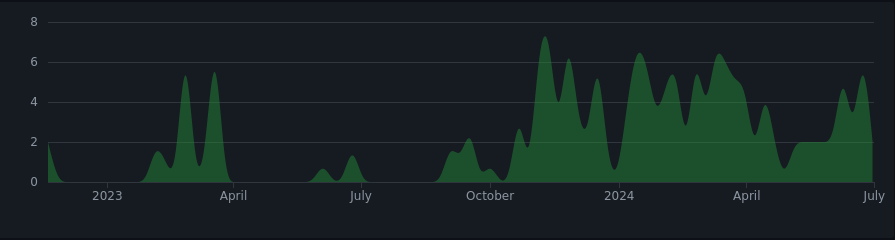
\includegraphics[width=0.9\textwidth,height=0.3\textwidth]{figs/objetivos/github.png}
    \end{center}
    \caption{Seguimiento de trabajo en GitHub}
    \label{fig:github}
  \end{figure}


\section{Plan de trabajo}
\label{sec:plantrabajo}

Finalmente, los pasos a seguir de este trabajo han sido: 
\begin{enumerate}
    \item Comienzo del trabajo. 
    \begin{itemize}
        \item Búsqueda del problema a desarrollar y análisis del estado del arte del uso de los drones en aplicaciones robóticas.
        \item Instalación de las diferentes librerías y aplicaciones de software. 
        \item Preparación de configuración de toda la infraestructura, teniendo un análisis y estudio de comunicaciones para poder comenzar con el desarrollo. 
    \end{itemize}
    \item Desarrollo: Una vez se tuvo listo toda la infraestructura tanto de comunicaciones como de librerías de software, se dio a pie el comienzo del desarrollo del código
        \begin{itemize}
            \item En primer lugar, se desarrollo un teleoperador sencillo del drone para ver el funcionamiento del vehículo y dicho comportamiento.
            \item Una vez finalizada la tarea del teleoperador, se comenzó con los algoritmos de percepción de detencción de carril mediante redes neuronales.
            \item Análisis y comparación de los resultados de los diferentes modelos que ofrece la red neuronal escogida con el propósito de tener la mejor solución. 
            \item El siguiente paso fue estudiar la posibilidad de tener un algoritmo de aprendizaje no supervisado llamado clustering para clasificar las diferentes lineas que aparezcan en el escenario de la carretera.
            \item Desarrollo del algoritmo de percepción junto con los dos puntos anteriormente mencionados.
            \item Con el fin del algoritmo de percepción, se comenzó el desarrollo de un controlador sencillo PID para ver el funcionamiento de la percepción y de la navegación en el vehículo. 
            \item A continuación, fue la programación del algoritmo de aprendizaje por refuerzo para el seguimiento del carril.
        \end{itemize}
    \item Evaluación: Se realizo la comparativa de los resultados obtenidos en el aprendizaje por refuerzo.
        
    \item Redacción de la memoria del trabajo para la documentación de todo el proceso de investigación realizado. 
\end{enumerate}


